\documentclass[letter,french]{report}
\usepackage[T1]{fontenc}
\usepackage[utf8]{inputenc} 
\usepackage{lmodern}
\usepackage{babel}
\usepackage[pdftex]{graphicx}
\usepackage{wasysym}
\usepackage{amsmath,amssymb}



\begin{document}
	\title{Devoir 1 IFT 3913}
	\author{Ludovic André et Gevrai Jodoin-Tremblay}
	\date{Remis le 5 Octobre 2017}
	\maketitle
	
	
	\subsection*{Description du logiciel}
	Ce logiciel affiche une interface usager simple à l'ouverture, très semblable
	à l'exemple d'interface usager de l'énoncé du travail pratique. Le bouton "Charger
	fichier" ouvre une fenêtre système permettant de sélectionner un fichier .ucd.
	Lorsqu'un fichier est choisi, il est \emph{parser} et ses éléments sont affichés dans
	les champs correspondants de l'interface.
	
	\subsection*{Ligne de compilation}
	Nous avons opté pour un \emph{makefile} histoire de rendre la compilation et l'exécution
	la plus facile possible sur les machines du DIRO. Un simple \emph{make} compile
	l'entièreté du logiciel et l'exécute. Pour voir les autres options, \emph{make help}
	explique les différentes commandes possibles.
	
	\section*{Conception}
	Pour notre travail, nous avons décidé de diviser notre projet en 3 différents
	paquets, comme on le voit dans le diagramme de paquet suivant.
	\newline 
	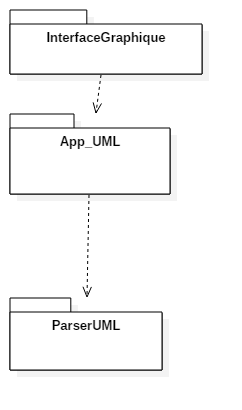
\includegraphics[scale=.3]{DiagrammePaquet.png}
	
	\subsection*{Parseur}
	Le parseur est inclus dans une seule classe statique, dont la seule méthode
	publique \emph{parse} prend une liste de \emph{String} correspondants aux lignes d'un
	fichier \emph{.ucd} et renvoie le \emph{UMLModel} correspondant. 
	
	Le \emph{parsing} est majoritairement fait avec des expressions régulières,
	principalement parce que la grammaire \emph{BNF} donnée dans l'énoncé si
	prêtait particulièrement bien. Ainsi, on découpe le texte en de plus en plus
	petits tronçons et ont créé les objets du paquet \emph{uml} directement.
	
	\subsection*{Interface Usager}
	
	
	\subsection*{Représentation des éléments UML}
	L'image suivante montre le diagramme de Classe de notre représentation UML.
	\newline 
	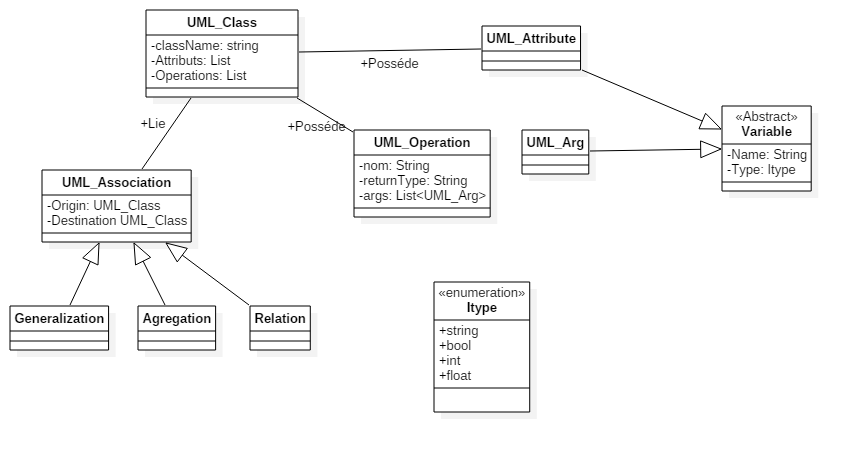
\includegraphics[scale=.3]{DiagrammeClasse.png}
	
	Ainsi, nous avons divisé en plusieurs classe notre représentation des éléments
	\emph{UML}. Tout en haut, la classe \emph{UMLModel} contient tous les autres
	éléments nécessaires. Nous avons une classe "UML\_Classe" qui représente les
	classes \emph{UML}. Ensuite cette classe possède des attributs et des opérations. Il faut aussi savoir que les méthodes ont aussi  des paramètres pour les opérations. Donc dans notre liste d'opération nous avons le nom de la méthode ainsi que ces paramètres. 
	
	De l'autre côté on a la
	classe "UML\_Association" qui elle a pour unique but de démontrer les liens
	entre 2 classes indiqués dans le diagramme UML.
	\newline
	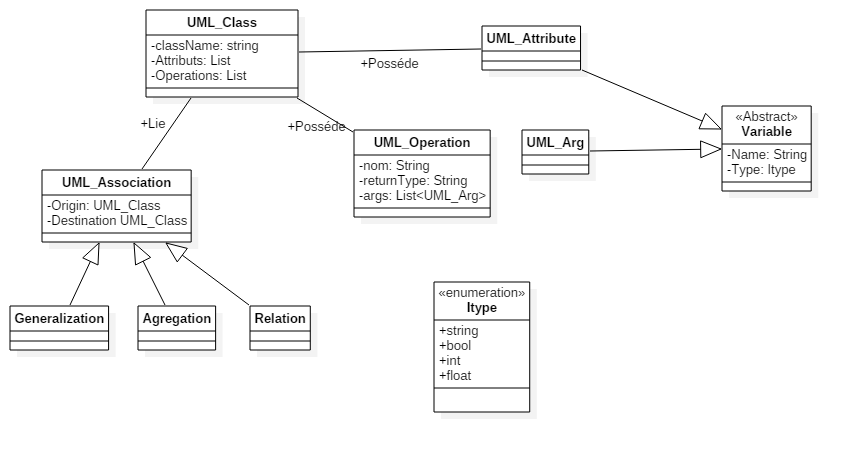
\includegraphics[scale=.4]{DiagrammeClasse.png}
	
	\section*{Implantation}
	
	\subsection*{Parseur}
	Le parseur est inclus dans une seule classe statique, dont la seule méthode
	publique \emph{parse} prend une liste de \emph{String} correspondants aux lignes d'un
	fichier \emph{.ucd} et renvoie le \emph{UMLModel} correspondant. 
	
	Le \emph{parsing} est majoritairement fait avec des expressions régulières,
	principalement parce que la grammaire \emph{BNF} donnée dans l'énoncé si
	prêtait particulièrement bien. Ainsi, on découpe le texte en de plus en plus
	petits tronçons et ont créé les objets du paquet \emph{uml} directement.
	
	\subsection*{MVC}
	Dans notre programme pour afficher les différents objets UML. Nous avons décidé de choisir un modèle MVC(Model-View-Controler). Dans la classe principale, nous avons notre contrôleur de vue. Ensuite on a divisé en deux classes. D’un côté nous avons notre contrôle dans UMLController qui contient toutes les méthodes qui seront utilisées quand on interagit avec notre interface. De l’autre, nous avons nos objets de notre interface graphique. De cette manière, on s’assure que notre application à une forte cohésion et un faible couplage. Si jamais on veut créer une nouvelle vue, on peut facilement le faire.
	
	
	
	
	
	\section*{Problèmes rencontrés}
Nous avons utilisé la librairie swing mais on s'est affronté à des problèmes. Nous avons eu des problèmes avec l'interface graphique. Notre application a eu de la misère à afficher toute l'information dans les cases si les noms des attributs,méthodes,associations ou sous-classes sont trop longs.

De plus, à un moment les éléments affichés d'une liste étaient limités et ne prenaient pas tout l'espace de la boîte. On a résolu ce problème en s'assurant que notre JScrollPane ait la propriété BorderLayout.Center.  

Par la suite, pour pouvoir gérer la sélection des multiples listes dans notre application, nous avons dû comme mentionner plus haut implémenter un MVC. Car c'était la seule solution qui nous permettait d'implémenter nos fonctions d'écoute pour toutes les listes dans l'application. Cela a eu comme conséquence que nous devions créer une méthode pour chaque liste de notre application qui génère une liste contenant les informations de la classe, la méthode, l'attribut, les sous-classes ou les associations.         

   
	
	
	
	\section*{Développement futur}
	Il serait très utile de pouvoir modifier un modèle UML directement à partir de l'interface,
	et permette l'exportation vers un fichier /.ucd/.
	
	
	
	
\end{document}
